%----------------------------------------------------------------------------------------
%	DOCUMENT CONFIGURATIONS
%----------------------------------------------------------------------------------------

\documentclass[a4paper,12pt]{report}
\usepackage[francais]{babel}
\usepackage[utf8]{inputenc}
\usepackage[T1]{fontenc}
\usepackage{ucs}
\usepackage{url}
\usepackage{graphicx}
\usepackage[table]{xcolor}
\usepackage[left=2.5cm,top=2cm,right=2.5cm,nohead,nofoot]{geometry}
\linespread{1.1}

\begin{document}


\setlength\parindent{0pt} % Removes all indentation from paragraphs


\begin{titlepage}
\begin{center}
\textbf{\textsc{UNIVERSIT\'E LIBRE DE BRUXELLES}}\\
\textbf{\textsc{Faculté des Sciences}}\\
\textbf{\textsc{Département d'Informatique}}
\vfill{}\vfill{}
\begin{center}{\Huge Analyse vidéo pour la détection, \\ suivi et reconnaissance de poissons}\end{center}{\Huge \par}
\begin{center}{\large \textsc{Della Monica} Simon, \textsc{Ooms} Aurélien, \textsc{Sonnet} Jean-Baptiste}\end{center}{\Huge \par}
\vfill{}\vfill{}
\begin{flushleft}{\large \textbf{Superviseur : Yann-A\"{e}l Le Borgne}}\hfill{}\end{flushleft}{\large\par}
\vfill{}\vfill{}\enlargethispage{3cm}
\textbf{Année académique 2012~-~2013}
\end{center}
\end{titlepage}




\tableofcontents
\newpage

\chapter{Introduction}

%----------------------------------------------------------------------------------------
%	Introduction
%----------------------------------------------------------------------------------------

\section{Motivation}

L'analyse logicielle vient de plus en plus appuyer le travail de tous ceux pour qui la récolte d'informations provient de processus d'acquisition numérique, i.e des vidéos enregistrées d'observations menées par des biologistes ou statisticiens.
 
L'usage de procédés automatisés permet le filtrage et l'analyse massive de données jusqu'alors fastidieuse à traiter. Données desquelles il est possible d'inférer ou d'appuyer des thèses selon les besoins.

Par exemple, l'analyse des déplacements individuels au sein d'un banc de poissons filmé pendant un longue période est une tache pour laquelle le passage par traitement informatisé apparaît comme nécessaire.\\

Le but de ce projet est d'ébaucher une solution logicielle d'analyse vidéo permettant l'automatisation du travail de détection et de suivi de poissons dans un milieu donné. 

\section{Approche et solution}

%----------------------------------------------------------------------------------------
%	SECTION 2
%----------------------------------------------------------------------------------------

\chapter{\'{E}tat de l'art}

Il existe un grand nombre d'approche pour traiter la détection et le suivi d'objet au travers de flux d'images. 

Il est nécessaire de prendre connaissance de ces différentes approches et leur évolution, ainsi que des bénéfices ou contraintes qu'elles induisent. D'autre part le sujet étant prolixe, nous limiterons ici l'exposé des méthodes de détection et de suivi à celles que nous avons utilisée ou celles qui nous sont, à un moment ou l'autre, apparues importantes pour traiter de la problématique qui nous occupe.

\section{Contexte, matériaux et questions}
Une vidéo est un flux, une succession d'images, dites  \textit{frames}. Le flux est dépendant de la fréquence de lecture/d'affichage, soit un taux en fps (\textit{frames per second}). 

Suivre une cible au long d'une séquence d'images, c'est définir et reconnaître une partie de l'image courante comme identique à la précédente, tout en lui autorisant des modifications (taille, position, couleur,...). Rétroactivement, c'est aussi reconstruire la trajectoire d'une cible dans la séquence d'images, cette approche se montrera pertinente pour la suite.\\

Le \textit{video tracking} ou suivi de cibles au sein d'une vidéo est le suivi de morceaux ciblés d'images au travers du flux duquel elles proviennent. C'est la tache automatisée qui consiste en la localisation, d'images en images, d'un groupe de pixels généralement en mouvement. \\

Si une cible apparait à l'oeil humain comme consistante alors qu'elle se meut dans son champs de vision, il en va tout autrement en \textit{computer vision}. En effet, à tout instant la consistance conférant son unité à la cible doit être déterminée, calculée et éprouvée pour qu'elle soit reconnue. 

Les parties traquées sont en fait chacune une quantité donnée de pixels, dans une espace restreint. Quantité à laquelle on concédera une identité en lui définissant/reconnaissant des attributs propres (variants et invariants). La cible sera alors contenue dans une \textit{région d'intérêt}, c'est-à-dire une sous-matrice d'une matrice plus grande que représente l'image toute entière.\\

\begin{figure}[hbtp]
\centering
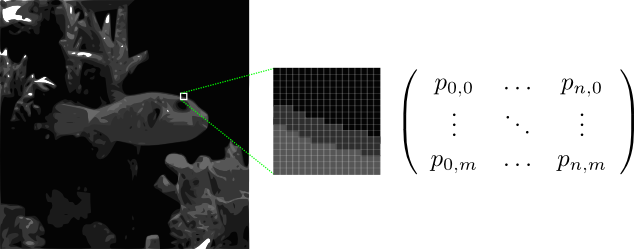
\includegraphics[scale=1]{figureImageMatrice.png}
\caption{Matrice de pixels}
\end{figure}


On perçoit plusieurs difficultés qu'il conviendra de maîtriser: l'unité de la cible et sa différenciation du fond, l'identité de celle-ci, malgré des modifications intrinsèques dans le flux d'images, la caractérisation et détermination du mouvement de la cible.\\
Deux problématiques fortement liées peuvent être dégagées\footnote{Video Tracking: A Concise Survey, E. Trucco, K. Plakas, IEEE Journal of Oceanic Engineering, Avril 2006}: le \textit{mouvement} et la \textit{correspondance}.

\subsection{La question du \textit{mouvement}}

	La question du mouvement comporte deux aspects: la détermination d'une cible comme mouvante et la caractérisation de ce mouvement.\\	
	
\subsubsection{Une cible mouvante}	
	L'approche qui semble la plus évidente pour cerner une cible en mouvement est sa différenciation avec ce qui apparait comme statique. 
	
	On supposera les objets d'intérêt et mouvant, comme appartenant à l'avant-plan (\textit{foreground}) et le reste, statique, comme appartenant au fond (\textit{background}). On parlera alors de \textit{soustraction du fond}.

\[F(\lambda_t) = \lambda_t - B_t\]	
où,
\begin{itemize}
\item[] $\lambda_t$ est une frame à l'instant $t$
\item[] Le \textit{foreground}: $F(\lambda_t)$ 
\item[] La \textit{background}, la matrice $B_t$\\
\end{itemize}

	La soustraction du fond peut se réaliser de différentes manières, mais elle doit pouvoir résister aux changements de luminosité, aux bruits et aux différentes variations de vitesse.
	De façon générale, l'extraction s'obtient en soustrayant de l'image courante une image de "référence", le fond.
	L'image de référence est actualisé à chaque étape, par accumulation pondérée et relativement à l'avant-plan extrait:
	
	$$\texttt{dst}(x,y)  \leftarrow (1- \alpha )  \cdot \texttt{dst}(x,y)+\alpha \cdot \texttt{src}(x,y)$$
	$$\texttt{if} \quad \texttt{mask} (x,y)  \ne 0$$
	où,	
	\begin{itemize}
	\item[] $\alpha$ est le \textit{facteur d'oubli}
	\item[] $\texttt{dst}(x,y)$ est le pixels de destination et $\texttt{src}(x,y)$ celui de l'image source.
	\item[] $\texttt{mask} (x,y)$ est une image binaire générée à partir de l'avant-plan extrait en $t-1$.
	\end{itemize}
	
	
	

\subsubsection{Un mouvement déterminé}		
	Le mouvement est caractérisé par une position d'origine (vecteur position), une direction (orientation vers un point de destination relativement a un référentiel) et une vitesse (obtenu en dérivant les coordonnées par rapport au temps).	
	L'enjeu est de parvenir déterminer que la position d'une cible à un instant $t$ est la résultante d'un mouvement, de cette même cible, initié en $t-1$.\\
	
	Plusieurs approche sont envisageables, notamment la définition du mouvement d'image de J.Shi et C.Tomasi .
	
	Le \textit{mouvement d'image}:
	$$I(x,y,t+\tau)=I(x-\xi(x,y,t,\tau),y-\eta(x,y,t,\tau))$$
	où
	\begin{itemize}
	\item[] $I_{t+\tau}$ est une image obtenue à partir d'un déplacement des points à l'instant $t$.
	\item[] Le vecteur de \textit{déplacement} $\delta = (\xi,\eta)$ est la quantité de mouvement. On perçoit l'insuffisance de la définition du déplacement $\delta$ quant aux multiples déplacements internes à la cible.\\
	\end{itemize}
	Le déplacement comme \textit{champs de mouvement affine}:
	$$\delta = D\texttt{x}+\texttt{d}$$
	où
	$D$ est la matrice de déformation et $d$ une translation sont donné comme:
	$$ D = \left( 
		\begin{array}{cc}
		d_{xx} & d_{xy} \\
		d_{yx} & d_{yy} \\ 
		\end{array} 
		   \right)
	$$
	Ce qui permet de poser pour un point $x$, centre d'une région d'intérêt de l'image $J_t$ son mouvement équivaudra au point $Ax + \texttt{d}$ de l'image suivante $J_{t+\tau}$, où $A = I + \texttt{D}$ et $I$ est la matrice identité donnée par:$$J_{t+\tau}(Ax + \texttt{d}) = J_t(x)$$\\
	La prédiction du mouvement sera donnée par l'estimation des paramètres de la matrice $D$ et du vecteur de déplacement $\texttt{d}$.\\
	
	
	
	Un autre approche plus courante est celle s'appuyant sur le concept de flux optique dont l'introduction est attribuée au psychologue James J. Gibson\footnote{\url{http://fr.wikipedia.org/wiki/Flux_optique}} . 
	
	Le flux optique (\textit{Optical Flow}) est décrit comme le modèle sous-jacent au mouvement visible d'un objet dans son contexte et relativement à l'observateur. Ce mouvement peut être estimé à partir d'une séquence d'images comme une suite de vitesses instantanées ou de déplacements discrets d'images.\\ 
	
	%l'une serait de cerner une région (autour de la cible) qui aurait une probabilité acceptable de contenir la cible à l'image suivante. La taille de la région serait donnée en fonction d'un mouvement prévu/attendu calculé sur une estimation précédente. Ce qui reviendrait à prédire et identifier une région dans laquelle l'élément ciblé aurait la plus grande probabilité de se trouver à l'image suivante. 
	
	%Estimer cette région à forte probabilité pourrait s'obtenir par le calcul de positions futures acceptables, pour chaque pixel définissant la cible (en prenant en compte l'historique récent de leurs mouvements).\\
	%Toutefois ce procédé semble rencontrer des difficultés d'une part lorsque la vitesse de la cible est sensiblement plus grande que le taux de frames du flux vidéo et d'autre part, lorsque la cible est de couleur relativement uniforme. Pour cerner le déplacement d'un pixel, il faut être en mesure de différencier la destination des attributs propres à l'origine et donc au pixel en mouvement, d'une façon certaine l'apparence uniforme empêche de faire apparaître les pixels comme mouvant, car la différenciation semble compromise. En ne focalisant plus sur un pixels, mais sur un groupes de pixels, la différenciation devient plus aisée, mais au détriment d'une sensibilité certaine et d'une définition précise du contour. C'est la problématique de l'ouverture, des block plus grands apparaissent plus sur et sont d'ailleurs moins sensible au bruit, mais offre moins de précisions\footnote{Block Matching for Object Tracking, A.Gyaourova, C.Kamath, S.C. Cheung, Department of Computer Science, University of Nevada, Reno, Center for Applied and Scientific Computing Lawrence Livermore National Laboratory, 2003}. \\
	% Un autre approche qui fait consensus est l'utilisation du \textit{filtre Kalman}\footnote{
%P. S.Maybeck, Stochastic Models, Estimation and Control. London U.K. Academic, 1979, vol. 1,2.}, celle-ci se révèle beaucoup plus performante.  

\subsection{La question de la \textit{correspondance}}

L'objectif est de reconnaître et identifier une cible d'une frame à l'autre. \\

\subsubsection{Critères d'intérêt}
Pour suivre une cible, on la compare au travers du flux d'images selon certaines \textit{unités de mesure}.
Ces unités de mesure sont façonnées au regard de la problématique traitée. Elles peuvent \^etre complexes et sont généralement hautement dépendantes des paramètres qui les composent.

Une unité de mesure est un ensemble des caractéristiques paramétrant l'objet cible, telles la position du centre de masse, l'aire, les coins, les contours ou encore l'historique des mouvements antérieurs. \\

La paramétrisation de la cible est capitale, car elle doit offrir des garanties sur l'identité de l'objet traqué. 
D'une image à l'autre, on doit pouvoir s'appuyer sur des critères robustes à l'évolution de la cible dans le flux d'image.


Il faut trouver des caractéristiques présentant des propriétés locales remarquables, c'est-à-dire des traits d'intérêts, stables ou \textit{invariants}, on parlera de \textit{features} de la cible.

Il existe diverses méthodes de détection de zones d'intérêts, chacune relative aux types de zones d'intérêts sur lesquels on souhaite baser l'analyse de la cible. Citons parmi les plus connu, l'algorithme de détection de coins de C. Harris et M. Stephens ou encore celui de J. Shi et C. Tomasi sur l'estimation qualitative des traits d'intérêts, mais aussi l'algorithme de détection de contours, \textit{Canny edge detection}, présenté par l'australien J. Canny en 1986.\\

\subsubsection{Fonction de mérite}
Une fois la caractérisation choisie, il faut établir une méthode de comparaison débouchant sur un coefficient de qualité sanctionnant l'estimation ou la prédiction de correspondance.\\

Une fonction de mérite, \textit{figure-of-merit}, est une fonction qui mesure la concordance entre les données et le \textit{modèle}, tout en considérant un choix particulier de paramètres.\\

En statistique fréquentielle, la fonction de mérite est généralement agencée de sorte que de petites valeurs obtenues représentent une concordance étroite. Tandis qu'une approche bayésienne choisirait une fonction de mérite de sorte à ce que des valeurs élevées représentent une meilleure concordance \cite{n}.

La fonction de mérite devra être telle qu'elle offre la meilleur façon de trouver l'extremum désiré en fonction des caractéristiques prédéfinies de la cible.\\

Elle devra aussi considérer que les données récoltées sont généralement bruitées.
Du fait que l'objet cible se modifie tout au long du flux d'images, la reconnaissance des critères comme correspondant comprend aussi leur différenciation du contexte/bruit. 

Par exemple, l'environnement où évolue la cible pourrait présenter l'une ou l'autre parcelle d'images assez ressemblante que pour passer comme identique au regard de l'unité de mesure définie.
De façon générale, pour outrepasser la pollution issue d'éléments parasites valides, il sera souvent nécessaire de mettre en œuvre plusieurs approches.
% existe des techniques de \textit{filtrage}, tel l'algorithme \textit{Conditional Density Propagation} \footnote{ Michael Isard and Andrew Blake, Int. J. Computer Vision, 29, 1, 5--28, (1998).
%$http://homepages.inf.ed.ac.uk/rbf/CVonline/LOCAL\_COPIES/ISARD1/condensation.html$ } ou d'isolation de la cible avec la méthode \textit{Gap-Mountain}\footnote{Moving Object Tracking in Video, Yiwei Wang and John Doherty and Robert Van Dyck, Department of Electrical Engineering, The Pennsylvania State University, National Institute of Standards and Technology}. 
%Ces techniques de filtrage de particules permettent aussi le tracking d'éléments dont le nombre varie au fil du temps \footnote{Filter-based Predictive Tracking for Robust Fish Counting, E. Morais, M. Campos, F. Pádua, R. Carceroni
%UFMG–Universidade Federal de Minas Gerais, Belo Horizonte, MG, Brasil} .

%\subsection{Problématique de l'identification}
%Le dénombrement et la classification des cibles peut être une démarche très utile. Par exemple, comptage des individus dans les fermes d’élevage ou classification des espèces en pleine nature, ou encore étude des relations prédateur-proie\footnote{One Fish, Two Fish, Butterfish,Trumpeter : Recognizing Fish in Underwater Video}.\\
%Techniquement, il est difficile de différencier des espèces de poissons en se basant uniquement sur une vidéo. En effet, plusieurs facteurs sont à prendre en compte :
%\begin{itemize}
%\item Déformations
%\item Décalage des couleurs
%\item Sédiments parasitant la visibilité
%\item Luminosité variable\\ 
%\end{itemize}
%
%Différents facteurs sont à prendre en compte lors de la tentative de reconnaissance :
%\begin{itemize}
%\item la cible peut apparaître de différentes manières devant l’objectif.\\ Pour résoudre ce problème, on utilise un algorithme de transposition au sein duquel on essaiera de faire correspondre la forme du poisson à , en tenant compte des différentes déformations.
%\item La déformation due à la distance par rapport à l’objectif.
%\end{itemize}


\section{Caneva}
Même s'il n'est pas de structure commune aux algorithmes existants pour la détection et le suivi de cible en mouvement, les étapes suivantes semble prévaloir pour beaucoup de ceux-ci.\\
\begin{center}
\begin{tabular}{ c c c c c c c } 
\cellcolor[gray]{0.9} Segmentation & $\rightarrow$ & \cellcolor[gray]{0.9} Extraction & $\rightarrow$ & \cellcolor[gray]{0.9} Analyse & $\rightarrow$ & \cellcolor[gray]{0.9} Suivi\\  
\end{tabular} 
\end{center}

\subsection{Segmentation}
A cette étape, il s'agit de dégrossir le matériau brut, de simplifier l'image en ne gardant que ce qui fait sens pour les opérations suivantes. L'objectif sous-tendant à toutes méthodes de traitement d'images étant de minimiser l'usage inutile de ressources computationnelles, la segmentation de l'image est une première approche pour ne plus focaliser que sur le signifiant. 

La segmentation est une opération de partitionnement de l'image en un certain nombre de segments. Cette opération est utilisée pour dégager des zones d'intérêts de l'image. Elle assigne une étiquette à chaque pixel de sorte que tous pixels identiquement étiquetés partagent des caractéristiques visuelles données (couleur, intensité, texture). Aussi tous les segments adjacents sont sensiblement différents suivant ces caractéristiques \footnote{\url{http://en.wikipedia.org/wiki/Segmentation_(image_processing)}}.\\

Il existe différentes méthodes de segmentation, certaines travaillent sur base de régions qu'elles accroissent, décomposent ou fusionnent, d'autres sur les contours, la classification ou le seuillage des pixels en fonction de leur intensité.\\
\subsubsection{Image binaire}
La méthode de segmentation la plus simple et la plus rapide est la création d'une image monochrome (aussi appelée \textit{binaire}) par seuillage: \`A partir de l'image originale convertie en niveaux de gris, on la transforme comparativement à une valeur seuil prédéterminée en une image binaire où chaque pixel prendra une des deux valeurs possibles.\\

Le niveau de gris d'un pixels $p$ est obtenu en calculant sa coloration moyenne: \[p_{\{r,g,b\}} =\frac{p_r+p_g+p_b}{3}\]\\

La transformation suivra la règle suivante:\\
soit une image $I$ de taille $m*n$, un seuil $T$ \textit{global} et $g(x,y)$ le niveau de gris du point $(x,y)$,

$$ \forall (x,y) \in I_{\{m,n\}}, (x,y) = \left\{ 
\begin{array}{rl}
1 &\mbox{si } g(x,y)>T\\
0 &\mbox{sinon}
\end{array} \right.
$$ 
Où les pixels appartenant à un objet de l'avant-plan sont étiquetés $1$ et ceux provenant du fond sont étiquetés $0$.\\ 

Cette approche grossière de seuillage peut être affinée par l'usage d'un histogramme de niveau de gris, offrant notamment la possibilité de segmenter l'image selon de multiples seuils.

Ou encore, plutôt que d'utiliser un seuil \textit{global}, il est possible de faire dépendre $T$ de propriétés locales du point évalué, comme par exemple de la valeur moyenne du niveau de gris de l'entourage du point considéré. On parlera d'un seuillage \textit{adaptatif} ou \textit{dynamique}.\\

L'image binaire peut, ensuite, être utilisée comme un masque permettant d'isoler des régions potentiellement intéressantes.

\subsubsection{Watershed}
L'algorithme de segmentation \textit{Watershed}, traduit par "ligne de partage des eaux", se base sur une interprétation tridimensionnelle de l'image, où un point est caractérisé par ses deux composantes spatiales et son niveau de gris.

De cette image, perçue comme un relief topographique, sera calculée la ligne de partage des eaux pour délimiter le bassin-versant, c'est-à-dire l'aire à l'intérieur de laquelle convergerait de l'eau hypothétiquement tombée. 

Trois types de points sont définis par cette interprétation:
\begin{itemize}
\item ceux appartenant à un minimum local.
\item ceux à partir desquels une goutte d'eau s'écoulerait inévitablement vers une minimum local précis. L'ensemble des points relatés à un même minimum constitueront un bassin-versant de ce minimum.
\item ceux à partir desquels toute goutte d'eau ruissellerait équitablement vers l'un ou l'autre minimum. L'ensemble des ces points forment topologiquement une crête, ils constituent la ligne de partage des eaux.\\
\end{itemize} 
 

Il existe plusieurs d'implémenter cet algorithme, parmi les plus communes: 
\begin{itemize}
\item selon la distance topographique d'un point au minimum le plus proche, à partir de chaque pixel de l'image, on suit le gradient jusqu'à atteindre un minimum, à l'image d'un ruissellement.
\item par inondation, où est simulé une montée progressive du niveau d'eau à partir des minima du relief.\\
\end{itemize}

La segmentation par ligne de partage des eaux donne de bons résultats dans l'extraction d'objet presque uniforme, mais conduit souvent à une sur-segmentation dû aux bruits et irrégularités locales. Une façon de pallier à ce désavantage est d'utiliser des marqueurs. Les marqueurs sont définis comme des composantes connexes appartenant soit à un objet d'avant-plan, soit au fond. La sélection des marqueurs à garder pourra être effectuée par simple estimation du niveau de gris et de la connectivité ou par une   


\subsubsection{Détection de contours}
Intuitivement, un contour est défini comme une suite de pixels contigus reflétant la frontière entre deux régions. 
La détection des contours permet alors de découper ou fusionner l'image en sous-régions.

En pratique, les principaux algorithmes de détection de contours, \textit{edge detection}, se basent sur l'étude des dérivées de la fonction d'intensité de l'image: le gradient, les extremums locaux et le passage par zéro du Laplacien. Le contour est obtenu par détection d'une discontinuité (changement abrupte d'intensité) et des similarités (selon des critères prédéfinis).\\

\begin{figure}[hbtp]
\centering
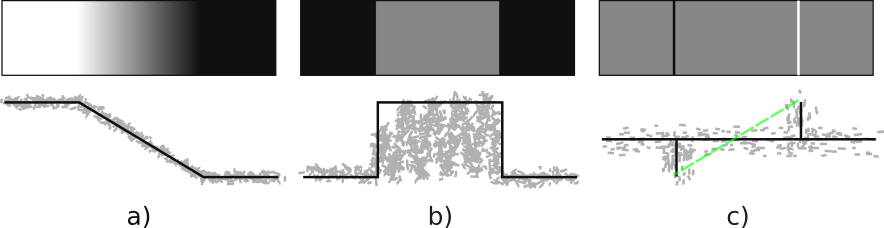
\includegraphics[scale=0.6]{figureDetectionDiscontinuities.png}
\caption{Détection de contours}
\label{fig:DetectionDiscontinuities}
\end{figure}

Dû notamment aux différentes méthodes d'acquisition, la frontière entre deux régions n'est pas toujours très contrastée ni exempte d'aucun bruit. De fait, elle apparaîtra généralement floutée et bruitée.\\ 
\`A partir d'une image en niveaux de gris, la frontière d'une région à une autre, représenté en \textit{a} dans la figure \ref{fig:DetectionDiscontinuities}, peut être \textit{idéalement} définie par une fonction rampe dont la longueur sera caractérisé comme le niveau de floutage de la frontière. 

Par l'étude de la dérivée première calculée en utilisant le gradient d'un point considéré (\ref{fig:DetectionDiscontinuities} \textit{b}), on peut déterminer si comparativement à un voisinage, on se trouve potentiellement sur un point du contour. 

De même, en évaluant la dérivée seconde par application du Laplacien (\ref{fig:DetectionDiscontinuities} \textit{c}), on peut:\begin{itemize}
\item en étudiant son signe, caractériser le point du contour comme appartenant à l'un ou l'autre coté de la frontière.
\item déterminer le milieu exacte de la frontière floutée. En calculant la droite imaginaire (\ref{fig:DetectionDiscontinuities} \textit{c}, ligne pointillée) joignant les extremums de la dérivée seconde, on obtient au passage à zéro le point médian.\\
\end{itemize}

Le filtre Canny est un des algorithmes les plus utilisés pour la détection des contours, il se base sur l'intensité et la direction du gradient. \\

\subsection{Extraction}

Des régions brutes délimitées par segmentation, il faut extraire les spécificités en vue d'effectuer les calculs souhaités.\\

L'idée est de réduire les cibles à leurs caractéristiques internes (pixels compris dans la région) et/ou externes (contours, frontières, coins) ayant une forte signifiance, puis de rassembler ces caractéristiques en descripteurs propre à chaque région. On parlera de \textit{descripteur} pour désigner l'ensemble des traits intéressants (\textit{features}) décrivant l'objet cible. 

Par exemple, une région pourrait être représentée par ses frontières et celles-ci serait décrites par des traits spécifiques (position relative des points du bord, périmètre, concavité, etc).
\\

Cette étape met en place un système de représentation des données en vue de les analyser. Autrement dit, on crée un système qui va compacter les données en des représentations utiles pour effectuer des calculs sur les descripteurs.\\

Le choix de ces traits est laissé libre, ils seront choisis relativement à la façon dont sera entrevue l'analyse des données. Par contre il est impératif que les traits caractéristiques forment des descripteur insensibles aux variations géométriques (homothétie, translation, rotation) ou photométriques (intensité).   
\subsubsection{Good feature to track}
Les «bons» traits à suivre sont ceux dont le mouvement peut être estimé de manière fiable.\\

J. Shi et C. Tomasi ont présenté\footnote{IEEE Conference on Computer Vision and Pattern Recognition (CVPR94) Seattle, June 1994} en 1994 leurs travaux sous l'intitulé \textit{Good Feature to Track}, l'article fait toujours autorité sur le sujet. 

Ils partent de l'évidence simple qu'aucun système de vision basée sur des traits d'intérêts ne peut fonctionner sans que des bons traits caractéristiques et robustes n'aient pu être préalablement identifiés. 

Ils proposent alors un critère de sélection de traits intéressants qu'ils précisent "optimal par construction" car basé sur la façon dont un système de suivi fonctionne.\\

Du constat qu'il n'existe de traits robustes à toutes épreuves et que même les bons traits peuvent se retrouver caché derrière un obstacle, cet article explique comment contrôler la qualité des traits caractéristiques de l'image.

Ce contrôle s'effectue pendant l'opération de suivi de la cible, par évaluation de la \textit{dissemblance}. 

La fonction de dissemblance, définie comme moyenne quadratique des traits, a pour rôle la quantification du changement d'apparence d'un trait entre l'image originale et l'image actuelle. Lorsque la dissemblance devient trop importante, le trait est abandonné.\\


Hypothèses concernant les traits intéressants à suivre:
\begin{itemize}
\item Luminosité constante: la projection d'un point conserve son apparence d'une frame à la suivante.
\item Mouvement court: un point ne bouge de beaucoup.
\item Cohérence spatiale: un point se déplace dans son voisinage.
\end{itemize}

\subsubsection{Detecteur de coins}
Un coin est un point intersection d'au moins deux arêtes de sens opposé.\\

Le \textit{Harris corner detector} est une méthode de détection de coins (traits d'intérêt) reconnu pour sa relative robustesse face aux bruits, aux variations de luminosité et aux variations géométriques. \\

L'algorithme, décrit par Harris et Stephens, fonctionne sur l'évaluation d'une fonction d'\textit{auto-corrélation} appliquée localement. 
En mathématique, l'auto-corrélation c'est corrélation croisée du signal par lui-même, cela permet de détecter des régularités, des motifs répétés au sein d'un signal.   

La fonction d'auto-corrélation, décrite par \cite{q} comme l'erreur quadratique moyenne (\textit{sum of squared differences}), mesure les changements locaux dûs à l'application d'un léger décalage dans chaque direction.\\
$$
E(x,y) = \sum_{u,v} \texttt{w}(u,v) \, \left( I(x+u,y+v) - I(u,v)\right)^2
$$
où
\begin{itemize}
\item[]$I$ est une image en niveau de gris.
\item[]$\texttt{w}(u,v)$ spécifie la taille de la fenêtre considérée, vaudra $1$ quand on se trouve dans la région d'intérêt, $0$ sinon.
\item[]$x$,$y$ est la quantité de déplacement dans une direction.
\item[]Une grande variation de $E$ dans la direction de $(x,y)$ dénote un trait d'intérêt.\\
\end{itemize}

\subsubsection{Flux Optique}

Une caméra filme des objets en mouvement dans un espace à trois dimensions, leur mouvement relatif est un champ de vecteurs à trois composantes. 

La scène filmée est projetée sur le plan, en deux dimensions, du flux vidéo. Dès lors, il est possible de définir un champ de vecteurs, le \textit{champ de vitesses projeté} \cite{r}. \\

Tout point $\textbf{X}$, réel filmé, possède un point $x$ d'une image dans le flux vidéo qui est le \textit{projeté} $p(\textbf{X})$ de vitesse $\textbf{V}$. 

Le flux optique est le vecteur $\vec v = dp(\textbf{X})\textbf{V}$.\\
 
L'estimation du mouvement est effectuée à partir de variations temporelles des intensités (niveau de gris) dans le flux d'images. Pour obtenir analytiquement le flux optique, on fait l'hypothèse que chaque point filmé a une intensité constante. On peut alors écrire cette dérivée comme $$\frac{d}{dt}I(t,x(t)) \equiv \frac{\partial I}{\partial x}V_x+\frac{\partial I}{\partial y}V_y+\frac{\partial I}{\partial t} \equiv \vec v \cdot \nabla I + \frac{\partial I}{\partial t}$$
où 
\begin{itemize}
\item[] $I(t,x,y)$ est une image en niveau de gris.\\
\end{itemize}
On a, sous l'hypothèse d'intensité constante, l'équation dite du \textit{flux optique}:
$$\vec v \cdot \nabla I + \frac{\partial I}{\partial t} = 0 $$ 
\begin{figure}[hbtp]
\centering
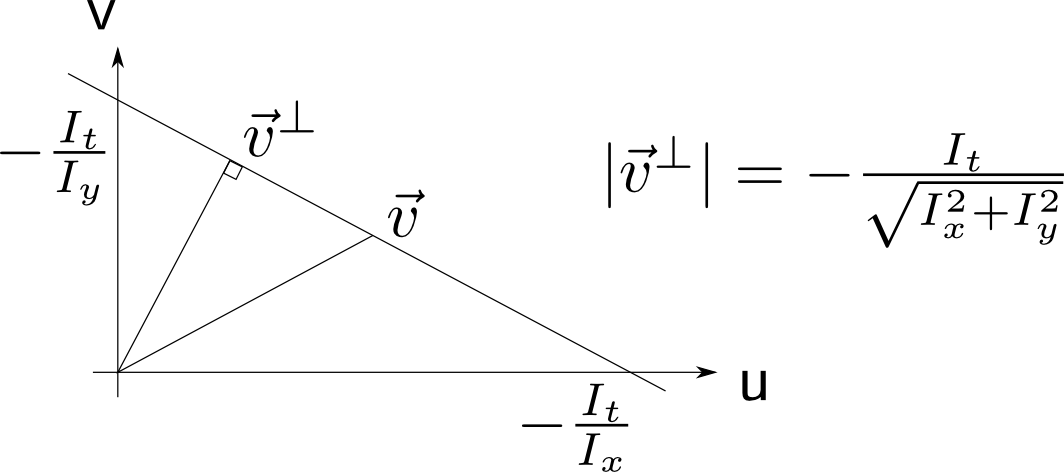
\includegraphics[scale=0.4]{figureOpticalConstraint.png}
\caption{Contrainte du flux optique}
\end{figure}

\subsection{Analyses}
\subsubsection{Matcher}
\subsubsection{Distance euclidienne}
\subsubsection{SURF}

\subsection{Suivi}


\section{Exigences}
Suite à ce qui a été énoncé, il est intéressant de dégager quelques exigences auxquels se devrait de répondre un système de tracking robuste. 
\begin{itemize}
\item \textit{Faux positifs, faux négatifs et résistance à la pollution d'éléments parasites}, il convient de ne suivre que ce qui doit l'être.
\item \textit{Fiabilité quand à une possible occlusion}, il est fort probable qu'à un moment ou l'autre, la cible sera occulté par un autre élément et réapparaîtra ensuite. Le tracking doit alors rester consistant.
\item \textit{Souplesse du tracking}, celui-ci doit pouvoir suivre des éléments aux vitesses variables.
\item \textit{Stabilité}, malgré tout, le suivi de la cible doit perdurer.
\end{itemize}


\chapter{Méthodes implémentées}

%----------------------------------------------------------------------------------------
%	Méthodes implémentées : Condensation
%----------------------------------------------------------------------------------------
\section{Conditionnal Density Propagation}
Afin de suivre un objet en mouvement au travers d'un flux vidéo, on doit être en mesure de déterminer à chaque \textit{frame} la position de la cible. 
Cette détermination est rarement exacte car elle s'appuie sur de nombreuses mesures, pour la plus part instables. 
La déformation de la cible, son occlusion, des changements de luminosité, etc, sont autant de mesures dont la propension à varier aléatoirement contribue à la génération de bruit dans la détermination de la cible.
On souhaiterait approcher l'hypothétique détermination réelle qui aurait été obtenue aux moyens de mesures idéales. Tout au plus, l'approche attendue devrait être en mesure de mettre en exergue le tout ou une partie de la cible comme n'appartenant pas au bruit.\\
Le processus de détermination se base sur un mouvement cyclique, partant d'un modèle donné dont la paramétrisation est issue d'observations antérieurs, on consolide ce modèle en évaluant sa pertinence à l'état présent, ce qui conduit à une prédiction sur l'état probable à l'étape suivant. 
On distingue alors deux phases, la \textit{prédiction} et l'\textit{observation}. La \textit{prédiction} est basée sur modèle affiné par les informations passées. L'\textit{observation}, ou phase de mesure, est la récolte d'informations sur l'état courant du système en vue de corriger la prédiction basée sur les mesures précédentes.\\
\begin{figure}[hbtp]
\centering
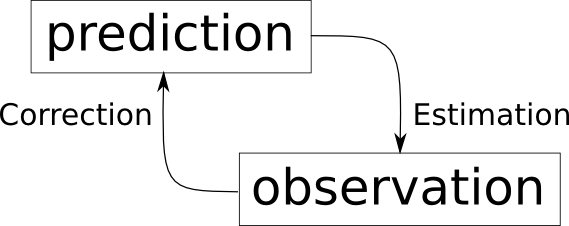
\includegraphics[scale=0.5]{figurePredictionObservationCycle.png}
\caption{Cycle de prédiction - observation}
\end{figure}

reconstruire la trajectoire d'attributs dans une séquence d'images \\
En probabilité, un processus stochastique vérifie la propriété de Markov si et seulement si la distribution conditionnelle de probabilité des états futurs, étant donné les états passés et l'état présent, ne dépend en fait que de l'état présent et non pas des états passés (absence de « mémoire »).
$P(\mathbf{x}_{t}|\mathcal{X}_{0:t})=P(\mathbf{x}_t|\mathbf{x}_{t-1})$
\subsection{Notation}
L'\textit{état} de l'objet $\mathbf{x}$ au temps $t$ est noté $\mathbf{x}_t$ et son historique est l'ensemble $\mathcal{X}_{0:t} = \{\mathbf{x}_0,...,\mathbf{x}_t\}$\\ 
De m\^eme, l'ensemble des \textit{features} (traits \textit{invariants}, aussi dit "les observations") est $\mathbf{z}_t$ et son historique $ \mathcal{Z}_{0:t}=\{\mathbf{z}_0,...,\mathbf{z}_t\}$\\
La dynamique stochastique du système (équation de transition) est entièrement donnée par $P(\mathbf{x}_t|\mathbf{x}_{t-1})$ (processus Markovien)
\paragraph{invariants}
caractéristiques locales de luminance, (photométrique) ou géométrique
\subsection{Dynamique du système}
\paragraph{Dynamique Stochastique}
L'état $\mathbf{x}$ est multidimensionnel et sa densité est plutot complexe.
Pour construire un  modèle dynamique, une connaissance \textit{a priori} du mouvement est nécessaire.
\paragraph{Observation}
Les observations $\mathbf{z}_t$ sont indépendantes entre-elles et vis-à-vis du processus dynamique:
$$P(\mathcal{Z}_{t-1},\mathbf{x}_t|\mathcal{X}_{t-1}) = P(\mathbf{x}_t|\mathcal{X}_{t-1})\prod_{t=1}^{t-1} P(\mathbf{z}_t|\mathbf{x}_t)$$
ce qui se réduit, considérant la condition mutuelle d'indépendance des observations, en
$$P(\mathcal{Z}_{t}|\mathcal{X}_{t}) = \prod_{i=1}^{t} P(\mathbf{z}_i|\mathbf{x}_i)$$
Le processus d'observation est alors défini en spécifiant la densité conditionnelle $P(\mathbf{z}_t|\mathbf{x}_t)$ pour chaque instant $t$
\paragraph{Propagation}
\`{A} partir des observations, la densité conditionnelle de l'état au moment $t$ est $P_t(\mathbf{x}_t) \equiv P(\mathbf{x}_t|\mathcal{Z}_t)$. Elle représente toute l'information de l'état pouvant être déduite de l'entièreté du flux de données.\\
Selon le théorème de Bayes, on déduit la règle de propagation de la densité de l'état dans le temps comme  
$$P(\mathbf{x}_{t}|\mathcal{Z}_{t}) = k_t P(\mathbf{z}_t|\mathbf{x}_t)P(\mathbf{x}_t|\mathcal{Z}_{t-1})$$
où $k$ représente une constante de normalisation ne dépendant pas de $\mathbf{x}_t$.\\
La densité \textit{a priori} $P(\mathbf{x}_t|\mathcal{Z}_{t-1})$ est une prédiction issue de la densité \textit{a posteriori} $P(\mathbf{x}_{t-1}|\mathcal{Z}_{t-1})$ provenant de l'étape précédente et à laquelle a été surimposé un pas de temps du modèle dynamique.
Pour atteindre cette densité \textit{a priori} tout en évitant un coût computationnel conséquent, celle-ci est approchée de façon récursive.

\subsection{\'{E}chantillonnage}
\subsubsection{Algorithme d'échantillonnage}
Il s'agit de retrouver un objet de paramétrisation $\mathbf{x}$ à partir d'une densité \textit{a priori} $P(\mathbf{x})$ en utilisant les données observées $\mathbf{z}$ d'une seule image.
La densité \textit{a posteriori} obtenue par l'application de Bayes est calculée récursivement  
\subsubsection{Séquence d'images temporelles}

\subparagraph{Contrainte de flot optique}
Méthode différentielle construite à partir d'une formulation différentielle d'un critère de corrélation.(ex Shi-Tomasi-kanade)
\subparagraph{méthode de corrélation}
Méthode basée sur des critères de corrélation (= fonction de similarité), 
estimer les déplacements
sensible au transformations géométriques (changement d'échelle, rotation, distorsion perspective) et photométrique de l'image


\chapter{Résultats expérimentaux}

%----------------------------------------------------------------------------------------
%	Résultats expérimentaux
%----------------------------------------------------------------------------------------


\chapter{Discussion}

%----------------------------------------------------------------------------------------
%	Discussion
%----------------------------------------------------------------------------------------


\chapter{Conclusion et perspectives}

%----------------------------------------------------------------------------------------
%	Conclusion et perspectives
%----------------------------------------------------------------------------------------



\bibliographystyle{apalike}
\bibliography{biblio}
\nocite{*}

\addcontentsline{toc}{chapter}{Bibliographie}

\end{document}